\chapter{Design Principles vs. Data}
In this chapter, we embark on a journey through the various stages of data visualization, focusing on geospatial data and its visualization. The goal of this demonstration is to create a \textbf{choropleth map} of California's counties, showing the most frequently affected counties when it comes to wildfires.

\section*{Data Preparation}
The goal of the first step of creating such a visualization is to decide what kind of data we need to display our desired graphic.

\begin{itemize}
    \item Calculate the fire frequency for each county: The choropleth map is going to color in the county's areas according to how many fires the data set has recorded.
    \item Next to the counties and their frequencies of wildfires we will be required to aggregate their locations on the map. The data set we have at hand provides us with latitude and longitude.
    \item Perhaps not every county is represented in the data set -- We therefore need to make sure to add these counties with zero incidents so the desired geomapping framework (\href{https://www.mapbox.com/}{Mapbox}) can handle our needs.
\end{itemize}

\section*{Select and Tailor Important Features}
After preparing the data on a general level the data needs to be cropped to its needs.

\begin{itemize}
    \item Implement a disambiguation process by cross-referencing county names with state identifiers. In the case of counties like ``Lake County'', which may exist in multiple states, it is crucial to include a state-level filter in the data processing pipeline. This ensures that only the ``Lake County'' located within the boundaries of California is included in the dataset used for the choropleth map.
    \item Cross-check the county names and their associated data against a reliable source, such as a government geographical database or API. This step can help to confirm that the data being visualized corresponds correctly to the intended locations within California.
\end{itemize}

\section*{Following Design Principles}
\subsection*{Choosing Appropriate Colors}
Effective choropleth maps for visualizing Californian wildfires should highlight accurate and meaningful spatial patterns, ensuring clarity and readability both in grayscale print and colored digital displays. Moreover, these maps must be crafted with colorblind-friendly design principles, ensuring accurate interpretation by a diverse audience, including those with color vision deficiencies. This approach guarantees that the maps are not only informative but also inclusive, providing a comprehensive understanding of wildfire distribution and impact across California \cite{doughertyDesignChoroplethColors2021}.

In this case the sequential color map ``plasma'' was used which is one of the out-of-the-box available colormaps from matplotlib. These default colormaps were made with all the common color design principles in mind, including colorblindness. The color map is also perceptually uniform, meaning that the colors are evenly distributed across the color spectrum. This is important because it ensures that the colors are not biased towards a certain color, which could lead to misinterpretation of the data \cite{bergmanRulebasedToolAssisting1995}. The chosen color map generally follows a linear sequential pattern which is what we want in our case as visual hierarchy is important when wanting to show frequency magnitudes of fires.

\subsection*{The Design Principles of Legends}
These following few points are important to keep in mind when designing a legend for a choropleth map:
\begin{itemize}
    \item The placement of the legend is crucial for the viewer to easily associate the labels with the corresponding data. Placing the legend below or parallel to the visualization ensures a clear connection between the two \cite{LegendsDataVisualization}.
    \item The decision on whether to include a legend title is based on the need to provide additional context to the visualization. If the title adds value and clarity to the chart, it should be included; otherwise, it can be omitted \cite{LegendsDataVisualization}.
    \item Directly labeling data representations instead of using a legend can enhance the understanding of the chart, as it reduces the cognitive load on the viewer. This principle aims to make the chart more intuitive and easier to interpret \cite{CarbonDesignSystem}. In the case of the choropleth map it is not possible to directly label the data in an aesthetically pleasing way as some counties are too small to fit the label in.
\end{itemize}

\subsection*{Showing Correct Scales}
The Choropleth map we try to visualize in this chapter should show which counties or therefore regions are most critically affected by wildfires. Depending on this task we need to think about how we want to scale the data. 

A common conception would be to assume that larger counties naturally have more wildfires, though that may not be true -- A county may be large but if the overall forest coverage is low, the rate of fires would most likely also be low. To counteract these underlying causalities we could scale the data \cite{doughertyNormalizeChoroplethMap2021}: In this case it would mean to divide the number of fires by the area of forest and thus display the rate of fires per acre through our color palette.

\begin{figure}[h]
    \centering
    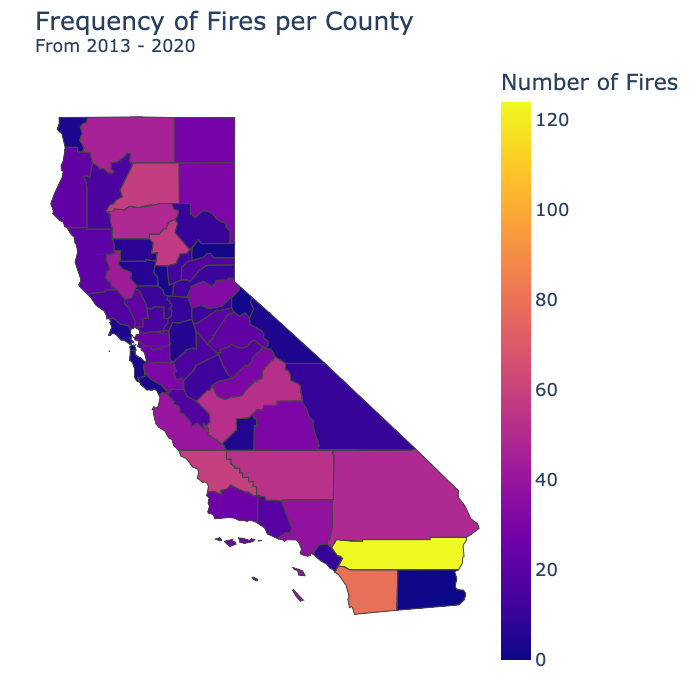
\includegraphics[width=0.6\textwidth]{Images/choropleth.png}
    \caption{Choropleth}
    \label{fig:enter-label}
\end{figure}